%% LyX 2.1.3 created this file.  For more info, see http://www.lyx.org/.
%% Do not edit unless you really know what you are doing.
\documentclass[12pt]{scrartcl}
\usepackage{lmodern}
\usepackage{lmodern}
\usepackage[T1]{fontenc}
\usepackage[latin9]{inputenc}
\usepackage{geometry}
\geometry{verbose,bmargin=1.5cm,lmargin=1.5cm,rmargin=1.5cm}
\usepackage{amsmath}
\usepackage{amssymb}
\usepackage{graphicx}
\usepackage{setspace}
\usepackage{wasysym}
\usepackage[authoryear]{natbib}
\doublespacing

\makeatletter

%%%%%%%%%%%%%%%%%%%%%%%%%%%%%% LyX specific LaTeX commands.
\newcommand{\lyxmathsym}[1]{\ifmmode\begingroup\def\b@ld{bold}
  \text{\ifx\math@version\b@ld\bfseries\fi#1}\endgroup\else#1\fi}

%% Because html converters don't know tabularnewline
\providecommand{\tabularnewline}{\\}

%%%%%%%%%%%%%%%%%%%%%%%%%%%%%% Textclass specific LaTeX commands.
\newcommand{\lyxaddress}[1]{
\par {\raggedright #1
\vspace{1.4em}
\noindent\par}
}

\@ifundefined{date}{}{\date{}}
%%%%%%%%%%%%%%%%%%%%%%%%%%%%%% User specified LaTeX commands.
\usepackage{lineno}

\makeatother

\begin{document}

\title{{\large{}Eco-evolutionary diversification of trait convergence and
complementarity in mutualistic networks }}


\author{{\normalsize{}Francisco Encinas-Viso$^{1,*}$, Rampal S. Etienne$^{2,**}$
and Carlos J. Meli�n$^{3,**}$}}

\maketitle

\lyxaddress{\textbf{\medskip{}
}\\
 \textbf{1}) NRCA \& Centre for Australian National Biodiversity Research,
CSIRO, GPO Box 1600 Canberra, Australia \\
 \textbf{2}) Groningen Institute for Evolutionary Life Sciences, University
of Groningen, The Netherlands \\
 \textbf{3}) Department of Fish Ecology and Evolution, Center for
Ecology, Evolution and Biogeochemistry, EAWAG, Swiss Federal Institute
of Aquatic Science and Technology, Switzerland\medskip{}
\\
 Keywords: Diffuse coevolution, specialization, sexual reproduction,
assortative mating, dispersal limitation, phylogenetic relatedness,
obligate mutualism, morphological constraints, individual based model.\medskip{}
\\
 Type of Article: Letters\\
 Number of figures: 6 in color; Number of tables: 1\\
 {*} Corresponding author: franencinas@gmail.com\\
 {*}{*} Joint last authorship}

\begin{linenumbers}

\newpage{} 
\begin{abstract}
  Mutualistic networks show high levels of convergence,
  complementarity and nestedness. Convergence and complementarity have
  been attributed to coevolutionary interaction selection under a
  phenotype matching scenario. It is not clear, however, whether
  phenotype matching fits empirical patterns better than a phenotype
  difference scenario. Here, we present a spatially and genetically
  explicit plant-animal trait diversification model combining the
  phenotype matching and phenotype difference model. Our model
  predicts high levels of convergence, complementarity, and
  nestedness. Comparing the predictions with observed levels of
  complementarity and convergence in an empirical plant-hummingbird
  mutualistic network, we find good predictions except for convergence patterns in plants. Our results
  indicate that combining the spatial structure of plant-animal trait
  diversification with population dynamics in a phenotypic difference
  model may alter predictions in a direction that is more in line with
  observations, and hence are important to be included in future
  studies of coevolutionary dynamics in mutualistic networks.

\newpage{}
\end{abstract}

\section*{Introduction}

Since Darwin's book ``On The Origin of Species'' \citep{darwin}, the
idea of coevolution, defined as reciprocal evolutionary trait change
between species, has sparked interest from biologists trying to
understand how species interactions generate trait changes. The first
clear indication of coevolution was Darwin's moth example
\citep{Darwin_orchids_book} showing that the long corolla from the
orchid \emph{Angraecum sesquispedale} could only be reached by a
pollinator species with a similar or larger proboscis
length. Following the moth and orchid mutualism model system, several
studies have modeled coevolutionary dynamics of a few species
\citep{Ferriere-2007,Law2001,Ferdy_2002,Gomulkiewicz-2003,Jones_Ferriere_amnat_2009},
particularly highly specialized (i.e. obligatory mutualists) systems
of plant-animal interactions, such as the fig-fig wasp mutualism
\citep{Bronstein-2006}.  These studies have determined the ecological
conditions for coevolutionary stable systems in highly specialized
plant-animal interactions \citep{Law2001,Jones_Ferriere_amnat_2009}

\citet{Janzen_coevolution_1980} argued that high specialization
between plants and animals was not the only example of coevolution,
but coevolution can also be the product of multiple-species
interactions, a term that he coined ``diffuse coevolution''. Diffuse
coevolution means that selection on traits is determined by the
interaction of more than two species and not only based on pairwise
interactions. This concept is based on the idea of ``syndromes'',
where, for example, plants have a set of traits that attract a
specific group of pollinator species with traits complementary to
those of the plants \citep{Jousselin_2003,guimaraes_coevol_2011}.
Evolutionary convergence, i.e. independent evolution of similar
features among different lineages of the same plant or animal
community may partly explain the formation of ``syndromes'' produced
by the presence of specific mutualist partner species
(\citet{Howe_1982};\citet{Waser_1996};\citet{Bascompte-Jordano-2007};\citet{Stayton_2008};\citet{Losos_2011}).

Theoretical studies suggest that evolutionary convergence and
complementarity are generated by coevolutionary interaction selection
driven by a ``phenotype matching model'' (Nuismer et al. 2005; Kopp
and Gavrilets 2006). For example, in highly specialized two-species
interactions such as the fig-fig wasp mutualism
\citep{Bronstein-2006}, plants coevolve with their most efficient
pollinator to strengthen the complementarity of their matching
traits. The phenotype matching model assumes that the probability of a
successful interaction decreases with increasing distance between the
phenotypes of the interacting individuals (Nuismer et al,
2012). Examples are plant and animal phenology (Jordano et al. 2003;
Olesen et al. 2010; Encinas-Viso et al, 2012) or proboscis and corolla
lengths (Agosta and Janzen 2005; Santamar�a and Rodr�guez-Giron�s
2007; Stang et al. 2007).

Only two theoretical studies have explored the importance of
coevolutionary selection and phenotype matching in the emergence of
convergence, complementarity and network structure in species-rich
mutualistic networks
\citep{Nuismeretal2012,guimaraes_coevol_2011}. \citet{guimaraes_coevol_2011}
studied a coevolutonary model with a fixed network structure and
showed that convergence in a one-dimensional trait may emerge as a
consequence of coevolutionary selection for a complementarity trait
between trophic levels. \citet{Nuismeretal2012} explored the
importance of coevolutionary selection in a multispecifies context to
study the emergence of convergence, complementarity and network
structure in mutualistic networks. They found that weak coevolutionary
selection produces little to no convergence but generates high
complementary. As coevolutionary selection intensifies, variation in
the trait values of animal and plant species is reduced and high
convergence emerges but complementarity decreases. Furthermore they
found antinested networks regardless of the strength of coevolutionary
selection.

\citet{Nuismeretal2012} also used an alternative model called
``phenotypic difference'' in which the success probability of an
interaction increases with the degree to which the animal trait
exceeds the plant trait as might be the case for fruit and beak size
in a dispersal mutualism (Lambert 1989; da Silva and Tabarelli 2000)
or proboscis and corolla length in some pollination mutualisms (Inouye
1980; Borrell 2007; Anderson and Johnson 2009; Anderson et
al. 2010). They showed that under the pheotype difference model
networks were more nested when coevolutionary selection was
weak. Furthermore, similar to the phenotypic matching model,
convergence increases with the strength of coevolution in the
phenotypic difference model (but only when interactions depend
strongly of phenotypes); however complementarity is weaker for
interactions mediated by phenotype difference than those mediated by
phenotype matchings. Taken together, these results suggest that it is
not trivial to simultaneously explain high degrees of convergence,
complementarity and nestedness in species-rich mutualistic networks as
observed in empirical data (\citet{Bascompte-Jordano-2007}. The
failure of succesfully explaining three patterns simultaneously may
also be a consequence of factors currently lacking in coevolutionary
models of mutualistic networks, such as {\small{}the role of genetics,
  gene flow, and assortative mating in plant-animal trait
  diversification
}(\citet{Gavriletsetal2000};\citet{deaguiar_2009};\citet{Schluter:2009};\citet{Doebeli_book};\citet{Seehausenetal_2014}),{\small{}
  and spatial structure and population dynamics. For example, although
  gene flow can be seen as an homogenizing factor, there is increasing
  evidence showing the importance of gene flow in the speciation
  process (Nosil, 2008) as well as the importance of spatial structure
}\citet{deaguiar_2009}{\small{}.  However, more importantly, there is
  no doubt that considering genetic processes (e.g. drift, selection)
  are essential to understand biodiversification patterns.  }In this
study we present an integrative model to study the patterns of
convergence, complementarity and nestedness in a model that includes
genetic processes, sexual reproduction, spatial structure, population
and trait diversification dynamics. Our model lies between a phenotype
matching and phenotype difference model, as an interaction can only
occur when the animal trait exceeds the plant trait, but the
probability of success does not increase with this difference.
Furthermore, we use a definition of convergence that accounts for
phylogenetic relatedness.

In contrast to previous studies, our model shows high levels of convergence,
complementarity and nestedness. Comparing these predictions to convergence
and complementarity patterns observed in a plant-hummingbird mutualistic
network, we find that the model is in agreement with observed level
of plant-animal complementarity and convergence for the hummingbird
community, but conflicts with convergence in the plant community.
Our results indicate that combining the spatial structure of plant-animal
trait diversification with population dynamics in a phenotype difference
model alter predictions in a direction that is more in line with observations,
and hence are important to be included in future studies of evolutionary
patterns in mutualistic networks. 


\section*{{\large{}Eco-evolutionary trait diversification in mutualistic networks}}

To study the effect of spatial structure and plant-animal trait diversification
on convergence, complementarity and nestedness in mutualistic networks,
we develop a spatial quantitative genetics model for plant-animal
interactions with overlapping generations. Individuals have fixed
genome size and we start with one plant and animal species with all
individuals having the same genetic composition at the outset (see
Figure 1 for the steps of the model). Following population demography
males and females individuals in both communities must be close enough
in spatial, genetic, and morphological space for an obligate mutualistic
interactions to occur (Figure 1 step B) and to produce offpsring with
a new genotype-phenotype after mutation, recombination and phenotypic
plasticity (Figure 1 step C, D and E). We follow the species definition
of \citet{Nei1983}, where a species is a group of interbreeding and
successfully reproducing individuals that are reproductively isolated
from other groups. In our model two individuals can mate successfully
if their genetic similarity value is larger than or equal to the minimum
genetic similarity value. Thus, speciation is defined as a group of
genetically related individuals, where two individuals in a sexual
population can be incompatible, but still conspecific as long as they
can exchange genes indirectly through other conspecifics \citep{deaguiar_2009,melian2010_plos}.
This is the definition of 'ring species' \citep{MoritzSchneider1992}.
Please refer to Figure 1, Table 1 and SI for a detailed explanation
of the terms included in the model and how we model population dynamics,
diversification dynamics, quantitative trait dynamics and neutral
locus evolution, respectively.


\section*{{\large{}Convergence, complementarity, nestedness and connectance}}


\subsection*{\textmd{Evolutionary convergence and complementarity}}

A focal species is considered to have convergent traits with another
species if it is phenotypically more similar to this other species
than to the genetically most similar species (the sister species)
(see figure \ref{fig:Evolutionary-convergence} and SI). The number
of convergences potentially increases with the number of species present.
For example, if we have ten species and we exclude one of them as
the sister species of the focal species, we have nine species to calculate
convergence. If we find that two out of nine species are phenotypically
similar enough to the focal species, we count two (out of nine,$\sim22\%$)
convergences. We repeat this by changing the focal species and calculate
the mean number of convergence events over all species. In contrast
to previous approaches that used the mean pair-wise difference between
traits of species \citep{guimaraes_coevol_2011} or the variance of
species traits in a guild as a proxy to predict convergence (i.e.,
large values weak convergence whereas small values of the variance
may indicate strong convergence, \citep{Nuismeretal2012}), our method
considering phylogenetic relatedness is that it excludes cases of
development of very similar trait values in sister species due to
shared evolutionary history and therefore it does not overestimate
convergence events. 

The condition for complementarity between two mutualistic partners
is simply that the phenotypic similarity between them, is larger than
some predefined phenotypic threshold value

We refer to the SI for a detailed explanation of phenotypic similarity
and mean genetic and phenotypic species similarity, and a precise
definition of complementarity and convergence in terms of these similarities. 


\subsection*{\textmd{Nestedness and connectance}}

To study the connection between convergence and complementarity with
network properties, we measured two topological properties of plant-animal
mutualistic networks: nestedness and connectance. We estimated nestedness
using the NODF algorithm developed by \citep{Almeida-neto_nodf} because
of its statistical robustness. NODF is based on standardized differences
in row and column fills and paired matching of occurrences. Connectance
measures the proportion of realized interactions among all possible
interactions in a network. It is defined as $C=\frac{k}{P*A}$, where
$k$ represents the number of realized interactions between plant
and animal species and $P$ and $A$ represent the number of plant
and animal species in the network, respectively \citep{Jordano-2003}.


\section*{{\large{}Simulations}}

We simulated equal population sizes for plants and animals with $J^{P}=J^{A}=1,000$
individuals. Genome size, $L$, of each individual was 150 loci.
Initial trait distributions for the plants, $Z^{P}=[z_{i}^{P}]$ and
animals, $Z^{A}=[z_{i}^{A}]$, were generated following equation 2
plus a normally distributed environmental effect, $\epsilon$, $\mathcal{N}(\mu_{\epsilon}=0,\sigma_{\epsilon}^{2}=1$).
To ensure plant mating conditions are met at the beginning of the
simulation all animal individuals have a higher phenotypic trait value
that the plant individuals.

Geographic distances between each pair of individuals $i$ and $j$
for the plants, $d_{ij}^{P}$, and animals, $d_{ij}^{A}$, were calculated
as follows: 1) Euclidean coordinates of a two-dimensional space ($x_{i},y_{i}$)
were sampled from a uniform distribution ($x_{i}=[0,1],y_{i}=[0,1]$)
for each individual for the plants and animals; 2) Using these coordinates
we calculated a matrix of relative Euclidean distances between the
individuals for the plants, $d_{ij}^{P}$, and animals, $d_{ij}^{A}$.
This procedure was repeated for each of the geographic distance matrices
($D^{PA},D^{P},D^{A}$) (See Table 1 and SI).

We ran 2,000 generations for each replicate for a total of 500 replicates,
where a generation is the update of the effective population size
($J^{P}=J^{A}=1,000$), i.e. the number of steps equal to the effective
population size. Steady-state was verified by checking the constancy
of speciation events during the last $1000$ generations. We calculated
convergence, complementarity, nestedness and connectance at steady-state.
Convergence and complementarity events were calculated for a whole
range ($[0.0,1.0]$) of their respective thresholds, $t_{conv}$ and
$t_{comp}$. We explored parameter combinations with mutation rate,
$\mu\in\{10^{-4},10^{-2}\}$, minimum genetic similarity, $q_{min}=0.97$,
maximum distance for finding a mate and disperse, $d_{max}\in\{0.1,0.3\}$,
and a maximum geographic distance to find a mutualistic partner, $d_{max}^{PA}=0.3$.
We implemented the model in Python (and tested in IPython \citep{ipython}).


\section*{{\large{}Confrontation to empirical data}}

We tested our model's predictions of convergence and complementarity
on a plant-hummingbird network with 38 hummingbird species and 133
plant species (\citet{Maglianesi_2014}). . To compute phenotypic
similarity we used empirical values of corolla length and bill length
from plants and hummingbirds, respectively (REF). . To compute phylogenetic
similarity for the hummingbirds we used a well resolved recently published
comprehensive phylogeny (McGuire et al, 2014) to obtain phylogenetic
relationships for 24 out of 38 hummingbird species; the remaining
14 species were not present in the phylogenetic tree. For the plant
species we constructed a phylogenetic tree using sequence data of
69 species from GenBank (data on rbcL, matK and ndhF genes collected
by PhyloGenerator using the option THOROUGH to allow also data from
close relatives if these relatives were not present in the community),
aligned them using MUSCLE (REF) and coonstructed the maximum likelihood
(ML) tree using RAXML (REF). We excluded 64 plant species from the
analysis (see Suppl. Information) because there was no sequence data
available or the phylogenetic relationships were not well resolved. 

We used the phylogenetic trees with their respective branch lengths
to calculate a genetic distance matrix among species. Using both phylogenetic
trees (hummingbirds and plants) we simulated nucleotide sequences
of 100 bp with the program SeqGen \emph{\citep{SeqGen_R_package}}
following the Jukes-Cantor model of molecular evolution. These simulated
sequences were then used to calculate the genetic distance matrix
using the R package \emph{seqinr }in R \citep{R_CRAN}. To compare
the convergence values obtained from the empirical data with our model
predictions, we generated 1000 replicates from the simulations (bootstrapping)
with each replicate containing the same number of plant and animal
species as the empirical data. Mean values as well 0.05 and 0.95 CI
were generated from these 1000 replicates. Complementarity and convergence
were calculated for each of the replicates across the whole range
of convergence, $t_{conv}$, and complementarity, $t_{comp}$, thresholds.
. We used a conservative definition for convergence in which not only
the sister species, but the 30\% most genetically similar species were
excluded.


\section*{{\large{}Results}}


\subsection*{Trait evolution}

Population dynamics and diversification dynamics changed plant and
animal community trait distributions (i.e. corolla and proboscis lengths)
with bimodal distributions being the most commonly produced patterns
across replicates (figure \ref{fig:Changes-in-trait}). At the species
level, a gradient of species phenotypes with common species presenting
lower mean and higher variance than rare species emerged. Mean and
variance of the trait values were correlated for most replicates (Spearman-$\rho$
> 0.41, $p$ < 0.05) and the distributions of abundance for plant
or animal species were highly skewed and significantly different from
a normal distribution (Lilliefors's test, all $p$ < 0.001). Abundance
predicted plant or animal mean species traits in approximately 70$\%$
of the replicates (Spearman-$\rho$ > 0.32, $p$ < 0.05) and trait
variance for all replicates (0.39 < Spearman-$\rho$ < 0.79, all $p$
< 0.05). Mean and variance of species trait values significantly
differed between common and rare plant or animal species (inset in
figure \ref{fig:Changes-in-trait}) suggesting a strong impact of
diversification by producing a gradient of species phenotypes in mutualistic
networks.


\subsection*{Convergence and complementarity}

Evolutionary convergence events occurred in all replicate simulations
(see equations SI-4 and SI-5 with an example of evolutionary convergence
events in animals and plants represented in figure \ref{fig:convergence-complementarity}).
Convergence events were heterogeneously distributed across species
with most events occurring between common species (0.42 < Spearman-$\rho$
< 0.89, all $p$ < 0.05). Evolutionary convergence occurred on average
in $17.3\pm6\%$ of all possible convergence events with more than
95\% of these events involving some of the three most common species.
These results show that evolutionary convergence is not randomly distributed
across pairs of species but highly aggregated during the diversification
process. Evolutionary convergence can also be visualized using a scatter
plot of the genotype-phenotype map for all pairs of individuals within
the plant and animal communities (see Figure SI-1 Supplementary Information).
As expected from equation \ref{eq:genetic_comp}, there is a positive
genotype-phenotype relationship. The scatter plot contains three main
clouds of points that consistently occur in our simulations for the
plants, \emph{P}, and animals, \emph{A}: 1) pairs of individuals of
the same species with high genetic ($q_{ij}>q_{min}$) and phenotypic
($p_{ij}>0.9$) similarity, 2) pairs of individuals of the same species
with genetic similarity below $q_{min}$ ($q_{ij}<q_{min}=0.97$)
and high phenotypic similarity ($p_{ij}>0.9$). These are incompatible
individuals of the same species for mating, yet with high phenotypic
similarity, $p_{ij}>0.9$, and 3) highly genetically dissimilar individuals
from different species, $q_{ij}\ll q_{min}$, but with the presence
of highly phenotypically similar individuals ($p_{ij}>0.9$). This
last category shows evidence of evolutionary convergence between species
in plants and animals. An increase in mutation rate increases the
genetic divergence between species, as expected, but it does not change
the genotype-phenotype relationship qualitatively (see Figure SI-1
Supplementary Information).

Evolutionary complementarity occurred with a similar frequency as
evolutionary convergence in each replicate (see equation SI-5 and
compare the initial with the final trait distributions in figure \ref{fig:Changes-in-trait}),
but with a larger variation ($20\pm18\%$). Connectance values were
consistently medium or high ($\overline{C}=0.5\pm0.07$, figure \ref{fig:nestedness}),
mostly larger than reported in empirical data where it ranges between
0.05 and0.25. Nestedness values were always high ($\overline{N}=69.97\pm13.4$
(figure \ref{fig:nestedness})), as observed in the empirical plant-pollinator
networks. Convergence, complementarity and nestedness did not show
signs of trade-offs and were uncorrelated across all replicates (0.08
< Spearman-$\rho$ < 0.27, all ~$p$ > 0.1) with the exception of
a positive correlation between trait complementarity and evolutionary
convergence in the plant community (Spearman-$\rho$ = 0.61, all $p$
< 0.05). Our results, using phylogenetic relatedness and phenotypic
similarity for the estimation of evolutionary convergence and complementarity
under weak coevolutionary selection, show evolutionary trait convergence
and complementarity in all our replicate simulations but with little
and large variation, respectively. These results suggest that in our
model, trait convergence in plant and animal communities is largely
independent or positively correlated with trait complementarity for
the animal and plant community, respectively. 


\subsection*{Comparison of model predictions with empirical data}

Our model predicts well plant-animal complementarity and convergence
for animals but not for plants in a empirical plant-hummingbird mutualistic
network (Figure 6). The observed proportion of complementarity events
for the empirical plant-hummingbird data is within the CI for a broad
range of values of the complementarity threshold, $t_{comp}$ (Figure
6a). Our model consistently predicts higher proportion of convergence
events than the observed proportion in the plant community (Figure
6b). Predictions in the proportion of convergence events quickly increase
for a high convergence threshold value both in the empirical data
and in our model predictions (red lines Figure 6b) and saturates around
the same observed values for medium and low convergent threshold values.
Predictions of the proportion of convergence events for the hummingbird
community are within the estimated CI for all the range of convergence
threshold values (Figure 6c). These results show that predictions
for plant-animal complementarity and convergence in the hummingbird
community are robust against a broad range of threshold values. 


\section*{{\large{}Discussion}}

Multispecific coevolution has been poorly studied so far due to its
complexity, which involves numerous processes and mechanisms in the
ecology and evolution of species interaction networks. Nevertheless,
there is accumulating empirical data (REFS) for and increasing interest
in understanding the drivers of multispecific coevolution in ecological
communities (REFS). . Our model comes closer to observed patterns
of complementarity and convergence in the plant-hummingbird community
than previous models.


\subsection*{The evolution of convergence and complementarity}

Previous studies have argued that evolutionary convergence is the
product of multispecific coevolutionary processes ('diffuse coevolution')\citep{Janzen_coevolution_1980,Thompson-2002,Jordano-2003,Bascompte-Jordano-2007}
and therefore convergence events are molded by similar ecological
(or niche) selective pressures. The model of \citep{Nuismeretal2012},
which studied a model of 'phenotype differences' has shown that for
weak coevolutionary selection trait values in animal and plant species
can be highly variable and non-convergent, but trait values of animal
and plants species show high complementarity (i.e. they are positively
correlated). However, strong coevolutionary selection decreases variation
in the trait values of animal and plant species increasing convergence
and simultaneously complementarity decreases (i.e. correlations between
traits of interacting species are weakened). Interestingly, the results
of \citet{guimaraes_coevol_2011} show that trait convergence may
in part emerge as a consequence of selection for a complementarity
trait between the plants and animals. This model, contrary to Nuismer
et al (2012), did consider background evolution (i.e. evolution driven
by other forces not related to mutualistic interactions \citet{guimaraes_coevol_2011},
which provides support to our results. 

Interestingly, the model of 'phenotype differences' considered here
has shown to make unlikely the evolution of convergence and complementarity
by coevolutionary selection \citep{Nuismeretal2012}. However, our
model shows that by considering a more realistic model of phenotype
differences in a more realistic setting gives results that are more
like the observations than the results of previous models. In other
words, it is possible to observe the evolution of both convergence
and complementarity. It remains to be seen whether the action of both
(selective an non-selective forces) and other models of plant-animal
interaction (e.g. 'phenotypic matching') will be able to generate
the observed patterns of high convergence, complementarity and nestedness
in species-rich mutualistic networks.

Non-selective forces underlying trait dynamics can produce convergence.
For example, \citet{Stayton_2008} simulated evolution along phylogenies
according to a Brownian motion model of trait change and demonstrated
that rates of convergence can be quite high when clades are diversifying
under only the influence of genetic drift. Furthermore, other types
of constraints in the production of variation can also lead to convergence.
If the variation produced is limited, then unrelated species are likely
to produce the same variation, which may then become fixed in the
population by genetic drift \citep{Stayton_2008,Losos_2011}. Developmental
constraints or the evolution of genetic networks by non-adaptive processes
may also be explanations for the convergence of traits \citep{Sole_convergence_selection_networks,Lynch:2007,Losos_2011},
but the role of developmental constraints or genetic networks in determining
convergence in species-rich mutualistic networks has yet not been
explored. For example, the tinkering of traits by evolutionary forces
largely affects developmental pathways (e.g. gene regulatory networks)
\citep{Sole_convergence_selection_networks}. Developmental pathways
are not static but can diverge through time randomly without substantially
affecting the phenotype \citep{Wagner:2008}. This concept, also called
developmental system drift (DSD) \citep{True_2001}, might play an
important role in the evolution of convergence in morphological traits
and it should be considered as another process where drift can act
\citep{Ohta_2002}, for example, by random wiring in gene regulatory
networks. Our results based on a method that excludes cases of the
development of a similar trait in related but distinct species descending
from the same ancestor show that additional constraints such as dispersal
limitation and assortative mating limit the production of variation
and lead consistently to convergence in distinct lineages in species-rich
mutualistic networks.

Evolutionary complementarity is also consistently observed in our
results but with a larger variation than convergence. Complementarity
is argued to be the main result of tight coevolution between mutualistic
species by mechanisms, such as trait-matching (e.g. corolla length-proboscis
length) \citep{Jordano-2003}. There is empirical \citep{anderson_johnson_2008}
and theoretical evidence \citep{Gomulkiewicz-2000} for coevolutionary
hot spots \citep{Thompson-1999}, which suggests that local selective
regimes can promote the coevolution of traits \citep{Gomulkiewicz-2000,Ferdy_2002,Gomulkiewicz-2003,Jordano-2003,Bronstein-2006,Thompson-2002,Thompson_2009,Jones_Ferriere_amnat_2009}.
In contrast, our results show that medium levels of complementarity
can emerge from relatively non-selective forces and constraints occurring
at several levels, from geographic limits to encounter partners and
disperse to the genetic and morphological constraints on producing
viable offspring. In addition, our model fitting show our predictions
fit well to the observed plant-hummingbird complementarity across
a broad range of complementarity threshold values (Figure 6). 

Our predictions are able to reproduce some observed patterns of convergence
and complementarity in a plant-hummingbird community. Observed convergence
values were close to those predicted by the model for the hummingbird
community, but we predicted more convergence values than those observed
in the plant community. According to previous models, fewer convergence
events could be indicative of weak coevolutionary selection processes
acting on the plant species. Although this is a possible explanation
for our overestimation of convergence, we think that our convergence
estimates may have been biased by the fact that we could not consider
all the plant species of the community ($\approx$ 50\%) only around
60\% of the hummingbird species. Our study is the first to quantify
and compare convergence and complementarity values from an empirical
dataset with model predictions and we believe this a major leap towards
the understanding of multispecific coevolution and community assembly.


\subsection*{The problem of calculating convergence}

One prominent problem in the literature is how to quantify convergence.
This problem is probably related to the lack of a rigorous or precise
definition of convergence (REFS). Previous studies (Nuismer et al,
Guimaraes et al) proposed different ways of doing this, but their measurements
of convergence do not consider phylogenetic relatedness. For example,
\citet{guimaraes_coevol_2011} measured convergence as ``the mean
pair-wise difference between traits of species at same trophic level''
considering all the species of the guild. \citep{Nuismeretal2012}
calculated the variance as a proxy to predict convergence (i.e., large
values weak convergence whereas small values of the variance may indicate
strong convergence). The main problem with these measurements that
ignore phylogenetic relatedness is that they will tend to overestimate
convergence events . Most definitions of convergence agree that it
is an evolutionary pattern in which ``similar phenotypes evolve \emph{independently}
in multiple lineages'' (Stayton, 2015). Therefore, it is important
to consider phylogenetic distance to correct for shared and therefore
dependent evolutionary history. Our model with our new measure of
convergence, which considers phylogenetic relatedness and phenotypic
similarity, shows that in the absence of abiotic selection trait convergence
and complementarity always evolve but with little and large variation,
respectively. Therefore, even with a more conservative estimate of
the number of convergence events, the results show that the modelled processes
(or background evolution sensu \citet{guimaraes_coevol_2011}) are
crucial for the emergence of these evolutionary patterns. 


\subsection*{The emergence of mutualistic network structure}

\citet{Nuismeretal2012} explored the connection between convergence
and complementarity to nestedness patterns in mutualistic networks.
They show that coevolutionary selection tend to decrease nestedness
and it generates even more strongly antinested networks when coevolutionary
selection increases by favoring the emergence of reciprocal specialization.
In contrast, nestedness values were very high in our model, as in
real mutualistic networks. Previous neutral models taking into account
ecological drift \citep{Krishna_2008,Canard_2012}, produced high
values of nestedness which suggests that random interactions and species
abundance distribution ('neutral forbidden links' \citep{Canard_2012}),
are determinants of the structure of mutualistic networks. Connectance
values obtained from our simulations are close to the predictions
of other neutral network models \citep{Canard_2012}. However, compared
to real mutualistic networks with similar diversity as ours (24 plant
and animal species on average), our connectance values ($\overline{C}=0.5$)
are higher than the reported webs ($C=0.28$) \citep{Olesen_Jordano_2002}.
Interestingly, \citet{Nuismeretal2012} found that only assuming coevolutionary
selection forces also leads to an increase in connectance. This means
that both basic genetic and ecological processes and coevolutionary
selection can increase connectance in mutualistic networks. The question
is why observed mutualistic webs have a lower connectance than those
predicted by our model and previous models. We conjecture that this
difference in connectance values might be due to different types of
forbidden links (i.e. biological constraints impeding plant-animal
interactions), such as phenology \citep{encinas_phenology_2012,Olesen-2008}
or environmental fluctuations that were not explicitly included in
our approach.

In summary, our results show the emergence of convergence, complementarity
and nestedness following basic genetic and ecological processes. Our
predictions fit well to the observed plant-hummingbird complementarity
and hummingbird convergence. In contrast to previous studies showing
antinested networks, we found highly nested values in agreement with
empirical mutualistic networks \citep{Bascompte-2003}. Our results
suggest that diversification dynamics combining ecological (demography
and dispersal limitation), population genetics (mutation, recombination,
assortative mating and drift) and morphological constraints may form
the basic processes producing the key patterns of mutualistic networks,
from trait convergence and complementarity to connectance and nestedness.


\section*{{\large{}Acknowledgments}}

We thank Martina Stang and Ole Seehausen for useful discussions. FEV
and RSE were supported by VIDI and VICI grants from the Netherlands
Organization for Scientific Research (NWO), awarded to RSE. CJM was
supported by the Swiss National Science Foundation (SNSF-project 31003A-144162).

\newpage{}
\bibliographystyle{evolution}
\bibliography{franeviso}


\newpage{}


\section*{Supplementary Information}


\section*{The model: evo-evolutionary trait diversification in mutualistic
networks}

To study the role of spatial structure and plant-animal trait diversification
on convergence, complementarity and nestedness, we start by considering
a landscape consisting of several individual plants (\emph{P}) and
animal pollinators (\emph{A}). We model obligate mutualism for both
partners and the number of individuals at each trophic level is fixed
and equal to the environmental carrying capacity for the given community.
Genetic, phenotypic and species composition change in time and space
due to population dynamics. At each time step replacement of dead
individuals are followed by the offspring of the same or another species
(the key terms and model steps are summarized in figure \ref{fig:Recombination}
and table 1, respectively). In this section we explain how we model
populations, traits, and diversification.


\subsection*{\textmd{Population dynamics }}

Our model is a stochastic individual-based model with overlapping
generations. The population consists of $J_{P}$ and $J_{A}$ haploid
gonochoric (i.e. separated sexes) individuals with an explicit genome
of size $L$ each and equal sex ratios at the outset. The genome of
each individual is composed of $L-1$ loci determining assortative
mating and one neutral locus. Both plant and animal population reproduce
sexually and are spatially structured. First an individual plant $k$
and an animal $k'$ are randomly removed (death). They are replaced
by reproduction. There are four conditions for producing viable offspring
for the plants and animals. These four conditions are 1) geography,
2) genetics, 3) obligate mutualism and 4) morphology: 
\begin{enumerate}
\item Geography: a female and a male individual within the plant and animal
populations are randomly chosen among all females and males within
a maximum distance, $d_{max}$ , of the dead plant $k$ and dead animal
$k'$. This requires two geographic distance matrices, one for plants,
$D^{P}$ = {[}$d_{ij}^{P}${]}, and one for animals, $D^{A}$ = {[}$d_{ij}^{A}${]},
containing all the pairwise distances. 
\item Genetics: to produce viable offspring the female and the male in the
plant and animal populations must have a genetic similarity value
of the assortative mating loci, $q_{\venus\mars}$, higher than the
minimum genetic similarity to have viable offspring, $q_{min}$, ($q_{\venus\mars}>q_{min}$).
This process reflects assortative mating and it requires two genetic
similarity matrices, one for plants, $Q^{P}$ = {[}$q_{ij}^{P}${]},
and one for animals, $Q^{A}$ = {[}$q_{ij}^{A}${]}, containing all
the pairwise similarity values. 
\item Obligate mutualism: in order to have a mutualistic interaction the
geographic distance between the female, $\venus$ (animal or plant),
and one of the two male animal or plant individuals, represented here
as $j$, must be lower than the maximum distance, $d_{max}^{PA}$,
($d_{j\venus}^{PA}<d_{max}^{PA}$). This requires one geographic plant-animal
distance matrix, $D^{PA}$ = {[}$d_{ij}^{PA}${]}, containing all
the pairwise distances. 
\item Morphology: the female plant need the presence of an animal pollinator
with a larger or equally-sized proboscis than the corolla of the plant,
thus the phenotype of the selected pollinator, represented here as
$j$, must satisfy $z_{\venus}^{P}\leq z_{j}^{A}$. This requires
two phenotype distributions, one for the plants, $Z^{P}=[z_{i}^{P}]$
and one for the animals, $Z^{A}=[z_{i}^{A}]$. This trait-mediated
interaction relationship is a variation on the ``phenotype differences''
model \citet{Nuismeretal2012}. 
\end{enumerate}
The offspring arising from this mating event will occupy the geographic
position of the just deceased individuals.


\subsection*{\textmd{Diversification dynamics}}

To quantify speciation events we calculate the genetic distance between
each pair of individuals based on the assortative mating loci. We
represent the genome of each individual by a sequence of $L-1$ loci,
where each locus can be in two allelic states, $+1$ or $-1$. The
assortative mating loci of each plant individual $i$ in a population
of size $J_{P}$ is represented as a vector: $S^{i}=(S_{1}^{i},S_{2}^{i},...,S_{L}^{i})$,
where $S_{u}^{i}$ is the $u^{th}$ locus of individual $i$. The
genetic similarity based on assortatove mating loci between individuals
$i$ and $j$ is calculated as the sum of identical loci across the
genome

\begin{equation}
q_{ij}^{P}=\frac{1}{L}\sum_{u=1}^{L}S_{u}^{i}S_{u}^{j}\label{eq:genetic_similarity-1}
\end{equation}
where $q_{ij}^{P}\in\{-1,1\}$ with the genetic similarity matrix,
$Q^{P}$ = {[}$q_{ij}^{P}${]}, containing all pairwise genetic similarity
values for plants (the same for animals, $Q^{A}$ = {[}$q_{ij}^{A}${]}).
The genome of the offspring is obtained by a block cross-over recombination
of a female genome, $S^{\venus}$, and a male genome, $S^{\mars}$,
where a locus $l$ in the genome of the parents is randomly chosen
partitioning the genome of each individual in two blocks. All genes
beyond that locus $l$ in either genome are swapped between the two
parents and eventually form two new genomes. One of the two new genomes
is randomly chosen for the offspring. The offspring's genome undergoes
mutations at mutation rate $\mu$. Figure \ref{fig:Recombination}
describes the recombination-mutation process.

At the beginning of the simulations all individuals are genetically
identical (all $q_{ij}^{P}$ and $q_{ij}^{A}$ = 1); hence they are
all able to mate and produce viable offspring regardless of their
spatial location. The genetic similarity between individuals of a
guild can be visualized as an evolutionary spatial graph \citep{melian2010_plos},
where nodes correspond to individuals and the edges correspond to
the geographic distances between a pair of individuals satisfying
the genetic similarity condition for mating, $q_{ij}^{P}(q_{ij}^{A})>q_{min}$.
The connectance of the graph will decrease when generations move forward
because of the processes described in the previous section: 1) spatial
constraints for mating driving assortative mating and dispersal limitation;
2) genetic divergence driven by the threshold for mating (incompatibilities),
mutation and recombination forming the genome of the offspring; 3)
obligate mutualistic interactions driven by spatial proximity of individuals
of the other guild, and 4) morphological constraints following the
phenotype differences scenario.

These four set of processes drive genetic divergence and speciation.
We followed the species definition of \citet{Nei1983}, which states
that species are groups of individuals that are reproductively isolated
and can interbreed to produce fertile offspring. In our model this
is realized through allowing two individuals to mate successfully
if their genetic similarity value is larger or equal to the minimum
value, $q_{min}$. Thus, speciation is defined as a group of genetically
related individuals, where two individuals in a sexual population
can be conspecific while also being incompatible, as long as they
can exchange genes indirectly through other conspecifics \citep{deaguiar_2009,melian2010_plos}.
This is the definition of 'ring species' \citep{MoritzSchneider1992}.

Genetic divergence will eventually produce the formation of two genetically
incompatible clusters of individuals, i.e. two species. This speciation
process, also called 'fission-induced' speciation, continues to form
more clusters and genetic divergence between individuals of different
species increases. However, the diversification dynamics will fluctuate
due to random extinctions (death of last individual of a species).
A stochastic balance between speciation and extinction is eventually
reached giving the final steady-state of the metacommunity.


\subsection*{\textmd{Quantitative trait dynamics}}

We model each individual plant and animal with a quantitative trait,
$z^{P}$ and $z^{A}$, respectively. The processes described in figure
\ref{fig:Recombination} govern two quantitative traits, one for each
guild: proboscis or bill length ($z_{i}^{A}$) in pollinators and
corolla length ($z_{i}^{P})$ in plants. The quantitative trait of
offspring is determined by the additive genetic effects of the genome
(i.e. no epistasis) after the process of randomly choosing one of
the two new genomes and mutation (figure \ref{fig:Recombination})
plus a normally distributed environmental effect, $\epsilon$, $\mathcal{N}(\mu_{\epsilon}=0,\sigma_{\epsilon}^{2}=1$)
\citep{guimaraes_coevol_2011}. The phenotype of the plant offspring
$i$ is $z_{i}^{P}=g_{i}^{P}+\epsilon$ and the genetic component
($g_{i}^{P}$) of the phenotype of offspring $i$ is

\begin{equation}
g_{i}^{P}=L+S_{o}^{i}\label{eq:genetic_comp-1}
\end{equation}
with $S_{o}^{i}=\sum_{u=1}^{L}S_{u}^{i}$. Hence $g_{i}^{P}$ is calculated
as the sum of alleles across the genome \citep{kondrashov_shpak_1998}
plus the number of loci to avoid negative trait values ($g_{i}^{A}$
is calculated similarly for animals). We assumed that the magnitude
of the influence (i.e., effect sizes) of any given locus on this quantitative
trait is equal across all the loci \citep{Seehausenetal_2014}. This
means that two individuals with a different combination of alleles
in the genome can express the same quantitative trait \citep{Losos_2011}.


\subsection*{\textmd{Neutral locus evolution}}

We considered a neutral locus to estimate genetic divergence among
species for the calculation of convergent events (see section ``Evolutionary
convergence''). The neutral locus is located at the end of the genome
at the position $L$ and it has $k$ possible allelic states. The
locus is completely unlinked from the rest of the genome that contains
the assortative mating loci. We used low mutation rates for this neutral
locus, $\mu_{neutral}=10^{-7}$ , and the $k$ allele mutation model
(i.e. model in which each allele can mutate to any of the other $k\lyxmathsym{\textendash}1$
possible alleles with equal probability (\citet{Hobanetal2013}).
We used the Cavalli-Sforza distance to calculate the matrix of genetic
distances among species (\citet{CavalliEdwards1967}).


\section*{Convergence, complementarity and nestedness}

Evolutionary convergence


\subsubsection*{\textmd{Phenotypic similarity}}

The phenotypic similarity for plants ($p_{ij}^{P}$) between individual
$i$ and $j$ is defined as 
\begin{equation}
p_{ij}^{P}=1-\frac{|z_{i}^{P}-z_{j}^{P}|}{z_{max}^{P}}\label{eq:phenotypic_sim-1}
\end{equation}
where $z_{i}^{P}$ and $z_{j}^{P}$ are the phenotypic similarity
values of $i$ and $j$, respectively, and $z_{max}^{P}$ is the maximum
value of the phenotype distribution, $Z^{P}$ . Thus, the elements
$p_{ij}^{P}\in\{0,1\}$ of the phenotypic similarity matrix, $\mathcal{P}^{P}$
= {[}$p_{ij}^{P}${]} represent all pairwise values for plants (the
same for animals, $\mathcal{P}^{A}$ = {[}$p_{ij}^{A}${]}).


\subsubsection*{\textmd{Mean genetic and phenotypic species similarity}}

We define evolutionary convergence as the similarity between average
species phenotypes from distantly related species. We assume that
two species are distantly related, in phylogenetic terms, if they
do not come from a direct common ancestor, i.e. they are not sister
species. To exclude sister species from the analysis we need to calculate
the mean genetic similarity among species of the same guild. The mean
genetic similarity between a plant species $k$ and a plant species
$l$ is

\begin{equation}
\hat{q}_{kl}^{P}=\frac{1}{n_{k}n_{l}}\sum_{i=1}^{n_{k}}\sum_{j=i}^{n_{l}}q_{ij}^{P}\label{eq:genetic_sim_species-1}
\end{equation}
where $q_{ij}^{P}$ is the genetic similarity between an individual
$i$ of plant species $k$ and an individual $j$ of plant species
$l$, and $n_{k}$ and $n_{l}$ are the absolute abundances of plant
species $k$ and $l$, respectively. The elements $\hat{q}_{kl}^{P}$
form the matrix $Q_{s}^{P}=[\hat{q}_{kl}^{P}]$ from which the sister
species of each species in the guild can be identified (The elements
for animals, $Q_{s}^{A}=[\hat{q}_{kl}^{A}]$, are calculated in the
same way as we did for the plants). To calculate evolutionary convergence
we need to know the average phenotypic similarity between two species.
We define phenotypic similarity between species $k$ and $l$ as

\begin{equation}
\hat{p}_{kl}^{P}=\frac{1}{n_{k}n_{l}}\sum_{i=1}^{n_{k}}\sum_{j=i}^{n_{l}}p_{ij}^{P}\label{eq:phenotypic_sim_species-1}
\end{equation}
which is analogous to the definition of eq. \ref{eq:genetic_sim_species-1},
but now considering phenotypes instead of genotypes. This will build
a species phenotypic similarity matrix $P_{s}^{P}=[\hat{p}_{kl}^{P}]$
(the species phenotypic similarity matrix, $P_{s}^{A}=[\hat{p}_{kl}^{A}]$,
is calculated analogously for the animals). We then focus on each
species in turn and exclude its sister species to avoid cases of parallel
evolution to calculate the number of convergences related to the focal
species. We define a focal plant species $k$ and a non-sister plant
species $l$ to be convergent if phenotypic similarity between them
is higher than between focal and sister species ($\hat{p}_{k,sister}^{P}<\hat{p}_{kl}^{P}$)
and higher than a certain phenotypic threshold value $t_{conv}$ ($\hat{p}_{kl}^{P}>t_{conv})$;
convergent species is calculated analogously for the animals).

Evolutionary complementarity


\subsubsection*{\textmd{Plant-animal interactions}}

In addition to the genetic and geographic constraints for mating,
we consider two other conditions for plants and animals: obligate
mutualism and morphological constraints. Obligate mutualism applies
to the plants and animals to reproduce but the morphological constraints
only apply to plants. We therefore need a geographic distance matrix,
$D^{PA}$, to describe the geographic distance between plant and animal
individuals. Plant-animal mutualistic interactions are here described
as follows: plants benefit from the presence of specific pollinators
that are able to pollinate them and animals benefit from the presence
of plants that provide resources for them. Thus, we have two extra
conditions for mating: 
\begin{enumerate}
\item Female plants need the presence of an animal pollinator (i.e., male
and female represented as $j$) within a close distance, $d_{j\venus}^{PA}<d_{max}^{PA}$.
The pollinator must have a larger or equally-sized proboscis than
the corolla of a plant, $z_{\venus}^{P}\leq z_{j}^{A}$. This corresponds
to a morphological constraint for individual interactions observed
between plant and pollinator species \citep{stang_2009_annbot,Stang_2006}. 
\item Animals need the presence of a plant (male or female represented as
$j$) within a close geographic distance, $d_{jk}^{PA}<d_{max}^{PA}$. 
\end{enumerate}

\section*{Tables}

\begin{table}


\protect\caption{Glossary of mathematical notation and parameter values}


\begin{tabular}{|c|c|c|}
\hline 
Notation  & Definition & Values \tabularnewline
\hline 
\hline 
$J^{P},J^{A}$  & Effective population size of plants (P) and animals (A) & 1,000 \tabularnewline
$d_{ij}^{P},d_{ij}^{A}$  & Geographical pairwise distance plants (P) and animals (A) & variable \tabularnewline
$d_{max}$  & Maximum geographical distance to mate and disperse & 0.3 \tabularnewline
$D^{P},D^{A}$  & Geographic distance matrix with all $d_{ij}^{P}$ and $d_{ij}^{A}$
values & variable \tabularnewline
$d_{ik}^{PA}$  & Geographical distance between plant $i$ and animal $k$ & variable \tabularnewline
$d_{max}^{PA}$  & Maximum geographical distance to find a mutualistic partner & 0.3 \tabularnewline
$D^{PA}$  & Geographic distance matrix with all the $d_{ik}^{PA}$ values & variable \tabularnewline
$q_{ij}^{P},q_{ij}^{A}$  & Genetic similarity between ind. $i$ and $j$ in (P) and (A) & variable \tabularnewline
$Q^{P},Q^{A}$  & Genetic similarity matrix with all the $q_{ij}^{P}$ and $q_{ij}^{P}$
values & variable \tabularnewline
$q_{min}$  & Minimum genetic similarity to have viable offspring & 0.97 \tabularnewline
$z_{i}^{P},z_{i}^{A}$  & Quantitative trait of ind. $i$ in (P) and (A) & variable \tabularnewline
$Z^{P},Z^{A}$  & Quantitative trait distribution in (P) and (A) & variable \tabularnewline
$p_{ij}^{P},p_{ij}^{A}$  & Phenotypic similarity between ind. $i$ and $j$ in (P) and (A) & variable \tabularnewline
$\mathcal{P}^{P},\mathcal{P}^{A}$  & Phenotypic similarity matrix with all the $p_{ij}^{P}$ and $p_{ij}^{A}$
values & variable \tabularnewline
$L$  & Size of the genome & 150 \tabularnewline
$g_{i}^{P},g_{i}^{A}$  & Genetic component of phenotype of offspring in (P) and (A) & variable \tabularnewline
$\epsilon$  & Environmental component of phenotype of offspring & $\mathcal{N}$(0,1) \tabularnewline
$\mu$  & Mutation rate per locus & $10^{-4}-10^{-2}$ \tabularnewline
$\hat{q}_{kh}^{P},\hat{q}_{kh}^{A}$  & Mean genetic simil. between species $k$ and $h$ in (P) and (A) & variable \tabularnewline
$Q_{s}^{P},Q_{s}^{A}$  & Species genetic simil. matrix with all $\hat{q}_{kl}^{P}$ and $\hat{q}_{kl}^{A}$
values & variable \tabularnewline
$\hat{p}_{kh}^{P},\hat{p}_{kh}^{A}$  & Mean phen. simil. between species $k$ and $h$ in (P) and (A) & variable \tabularnewline
$P_{s}^{P},P_{s}^{A}$  & Species phen. simil. matrix with all $\hat{p}_{kl}^{P}$ and $\hat{p}_{kl}^{A}$
values & variable \tabularnewline
$\hat{p}_{kh}^{PA}$  & Mean trait similarity plant species $k$ and animal species $h$ & variable \tabularnewline
$P_{s}^{PA}$  & Phenotypic simil. matrix with all $\hat{p}_{kh}$ values & variable \tabularnewline
\hline 
\textit{\footnotesize{}\textsuperscript{h}conv} & Phenotypic threshold to calculate convergence events & variable\tabularnewline
\textit{\footnotesize{}\textsuperscript{h}comp} & Phenotypic threshold to calculate complementarity events & variable\tabularnewline
\end{tabular}
\end{table}


\end{linenumbers}

\newpage{}


\section*{Figures}

\begin{figure}
\begin{centering}
\includegraphics[scale=0.5]{Figures/IBModel6.eps}
\par\end{centering}

\protect\caption{The death-birth cycle per time step. Individuals are represented as
filled circles and blue tones represent variation of phenotypes. (A)
an individual $k$ is randomly selected to die and leaves an empty
location in the landscape. (B) a female individual, $\venus$, is
randomly selected among all females satisfying the condition $d_{k\venus}<d_{max}$.
We then choose randomly a male, $\mars$, among all males satisfying
$d_{k\mars}<d_{max}$ and $q_{\venus\male}>q_{min}$ with $q_{min}$,
the minimum genetic similarity required for mating. In addition to
these two constraints, two more are required to complete mating. For
the condition of obligate mutualism, the geographic distance between
the female (animal or plant), and an animal (or plant) individual
$j$, must satisfy $d_{j\venus}^{PA}<d_{max}^{PA}$. Finally, female
plants need the presence of an animal pollinator with a larger or
equally-sized proboscis than the corolla of the female plant, thus
individual pollinators represented as $j$, must satisfy $z_{\venus_{P}}\leq z_{j_{A}}$.
In (C) and (D) we calculate the genome of the new offspring once these
constraints are satisfied. (C) Genomes are composed of $L$ loci where
each locus can be in two allelic states ($-1,\,1$) and undergo block
crossover recombination between female (dark gray) and male (black).
A position $l$ in the genome of the parents is randomly chosen partitioning
the genome in two blocks. All genes beyond the $l$ locus in either
organism's genome is swapped between two parents and two new genomes
are formed. (D) One of the two new genomes is randomly chosen for
the offspring $i$, $S_{o}^{i}$, and it might undergo mutation (light
gray). (E) The phenotype expression of offspring $i$ is $z_{i}=g_{i}+\epsilon$
with $g_{i}=L+S_{o}^{i}$ and $\epsilon$ are the genetic and environmental
component of the phenotype, respectively. (F) The offspring $i$ occupies
the site of the dead individual $k$. \label{fig:Recombination}}


\end{figure}


\begin{figure}
\begin{centering}
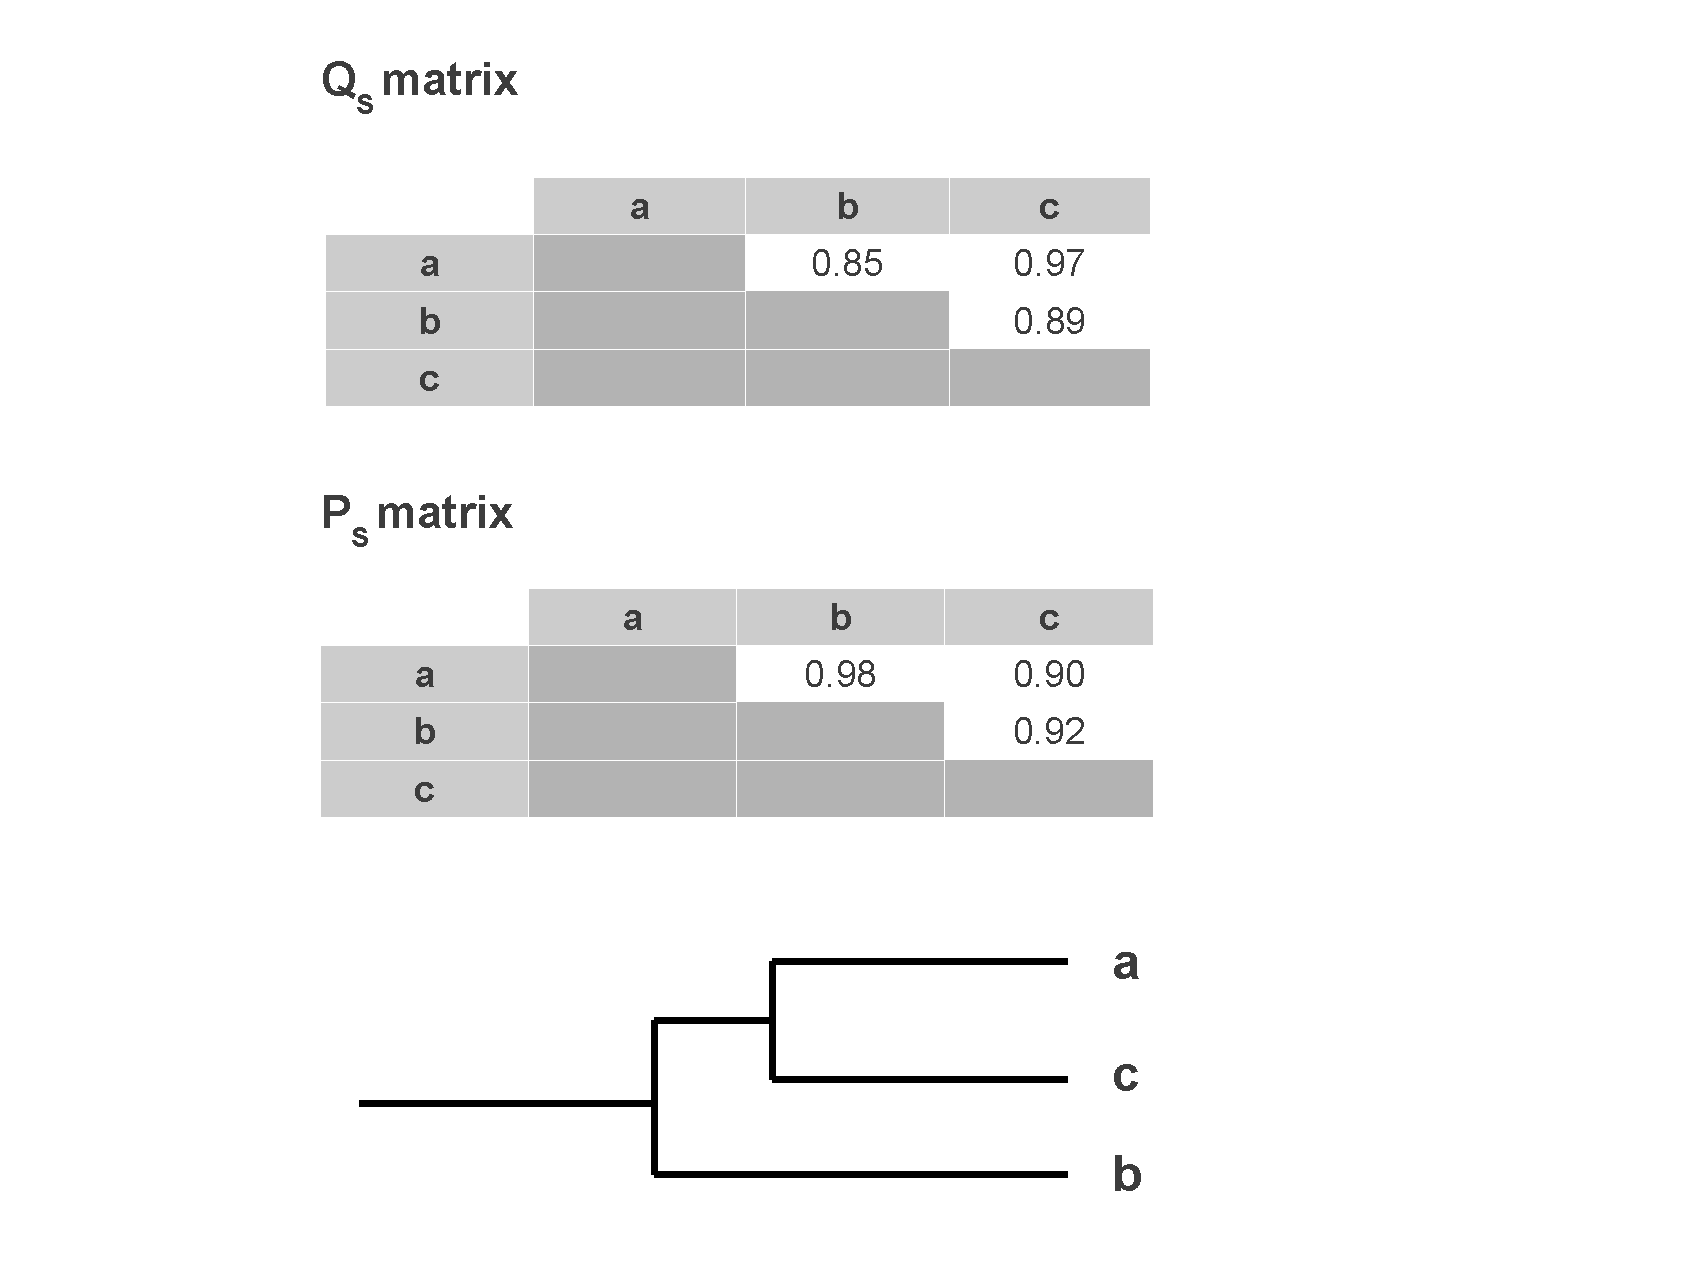
\includegraphics[scale=0.6]{Figures/convergence.eps}
\par\end{centering}

\protect\caption{A simple example of evolutionary convergence using species $a$, $b$
and $c$. The upper matrix ($Q_{S}=[\hat{q}_{kl}]$) shows species
$a$ and $c$ are genetically closely related, $\hat{q}_{ac}=0.97$,
while genetically distant from species $b$ ($\hat{q}_{ab}=0.85$,
$\hat{q}_{cb}=0.89$). A clear description of these genetic relationships
can be represented with a cluster tree or dendrogram, as shown in
the lower part of the figure. Thus, we establish that species $a$
and $c$ are sister species. The species phenotypic similarity matrix,
$P_{S}=[\hat{p}_{kh}]$ shows that species $a$ and $b$ are phenotypically
highly similar ($\hat{p}_{ab}=0.98$) and highly genetically dissimilar
($\hat{q}_{ab}=0.85$) (i.e. more than the average intraspecific genetic
similarity or sister species $~0.97$), indicating an event of evolutionary
convergence.\label{fig:Evolutionary-convergence}}


\end{figure}


\begin{figure}
\begin{centering}
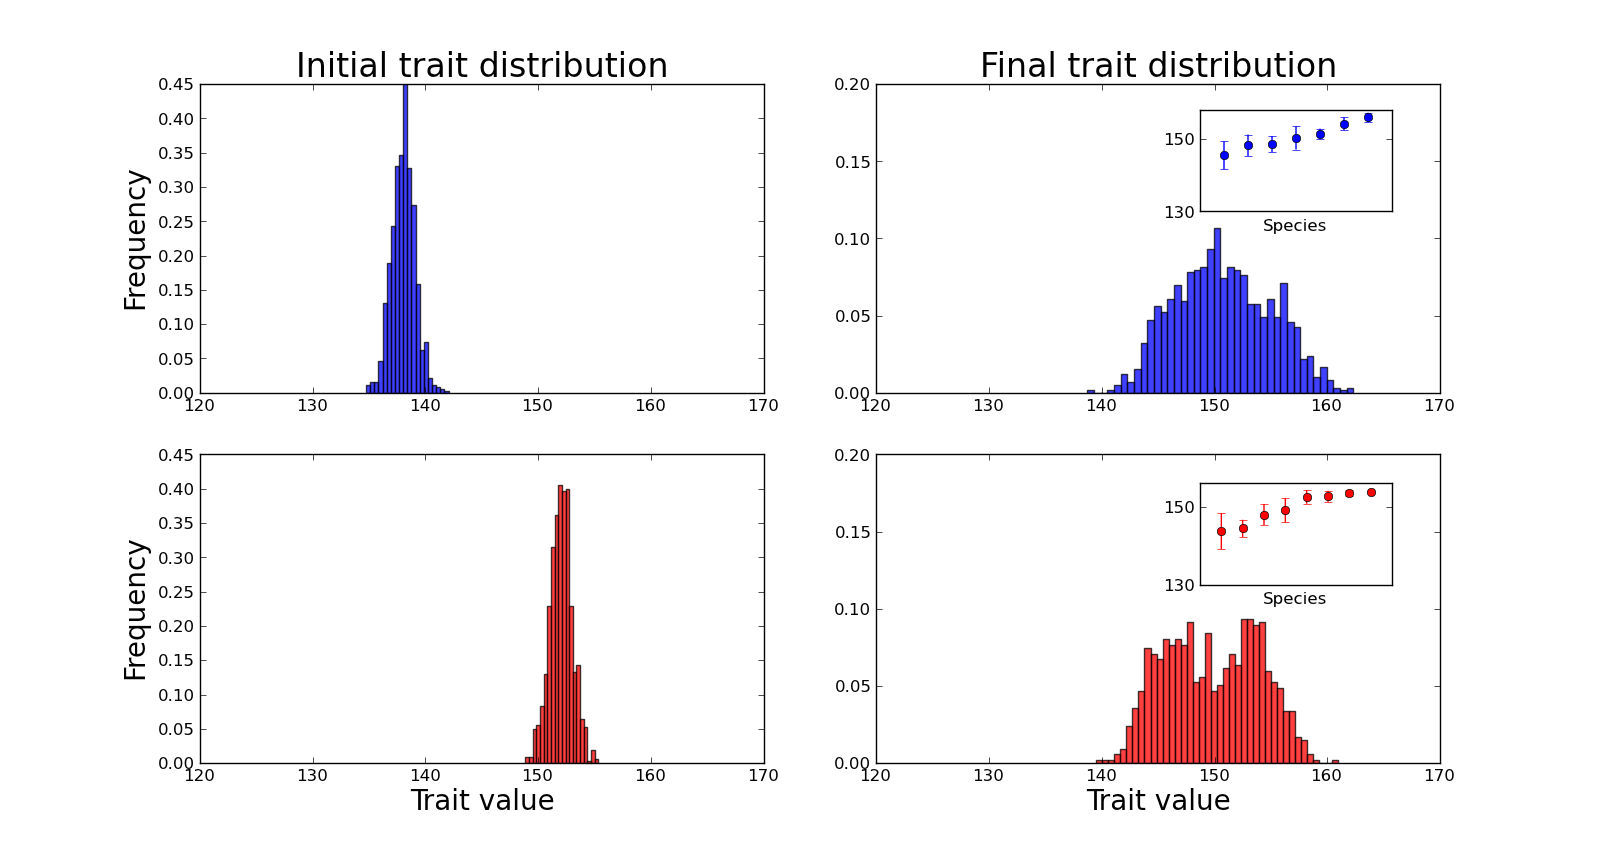
\includegraphics[scale=0.4]{Figures/trait_dist_2.eps}
\par\end{centering}

\protect\caption{Changes in trait distribution of plants (top, blue) and animals (bottom,
red). Left and right panels show the initial and final trait distribution,
respectively. The insets in the right panels show the mean trait and
standard error for each species sorted from the most common to the
most rare. Initial trait distributions changed towards higher variance,
and in most replicates, towards bimodal distribution in both guilds.
Shown is the outputs from one replicate with parameters values\textbf{
$q_{min}=0.97$, $d_{max}=d_{max}^{PA}=0.3$, $\mu=5\times10^{-3}$
and $J_{P}=J_{A}=1,000$.\label{fig:Changes-in-trait}}}
\end{figure}


\begin{figure}
\begin{centering}
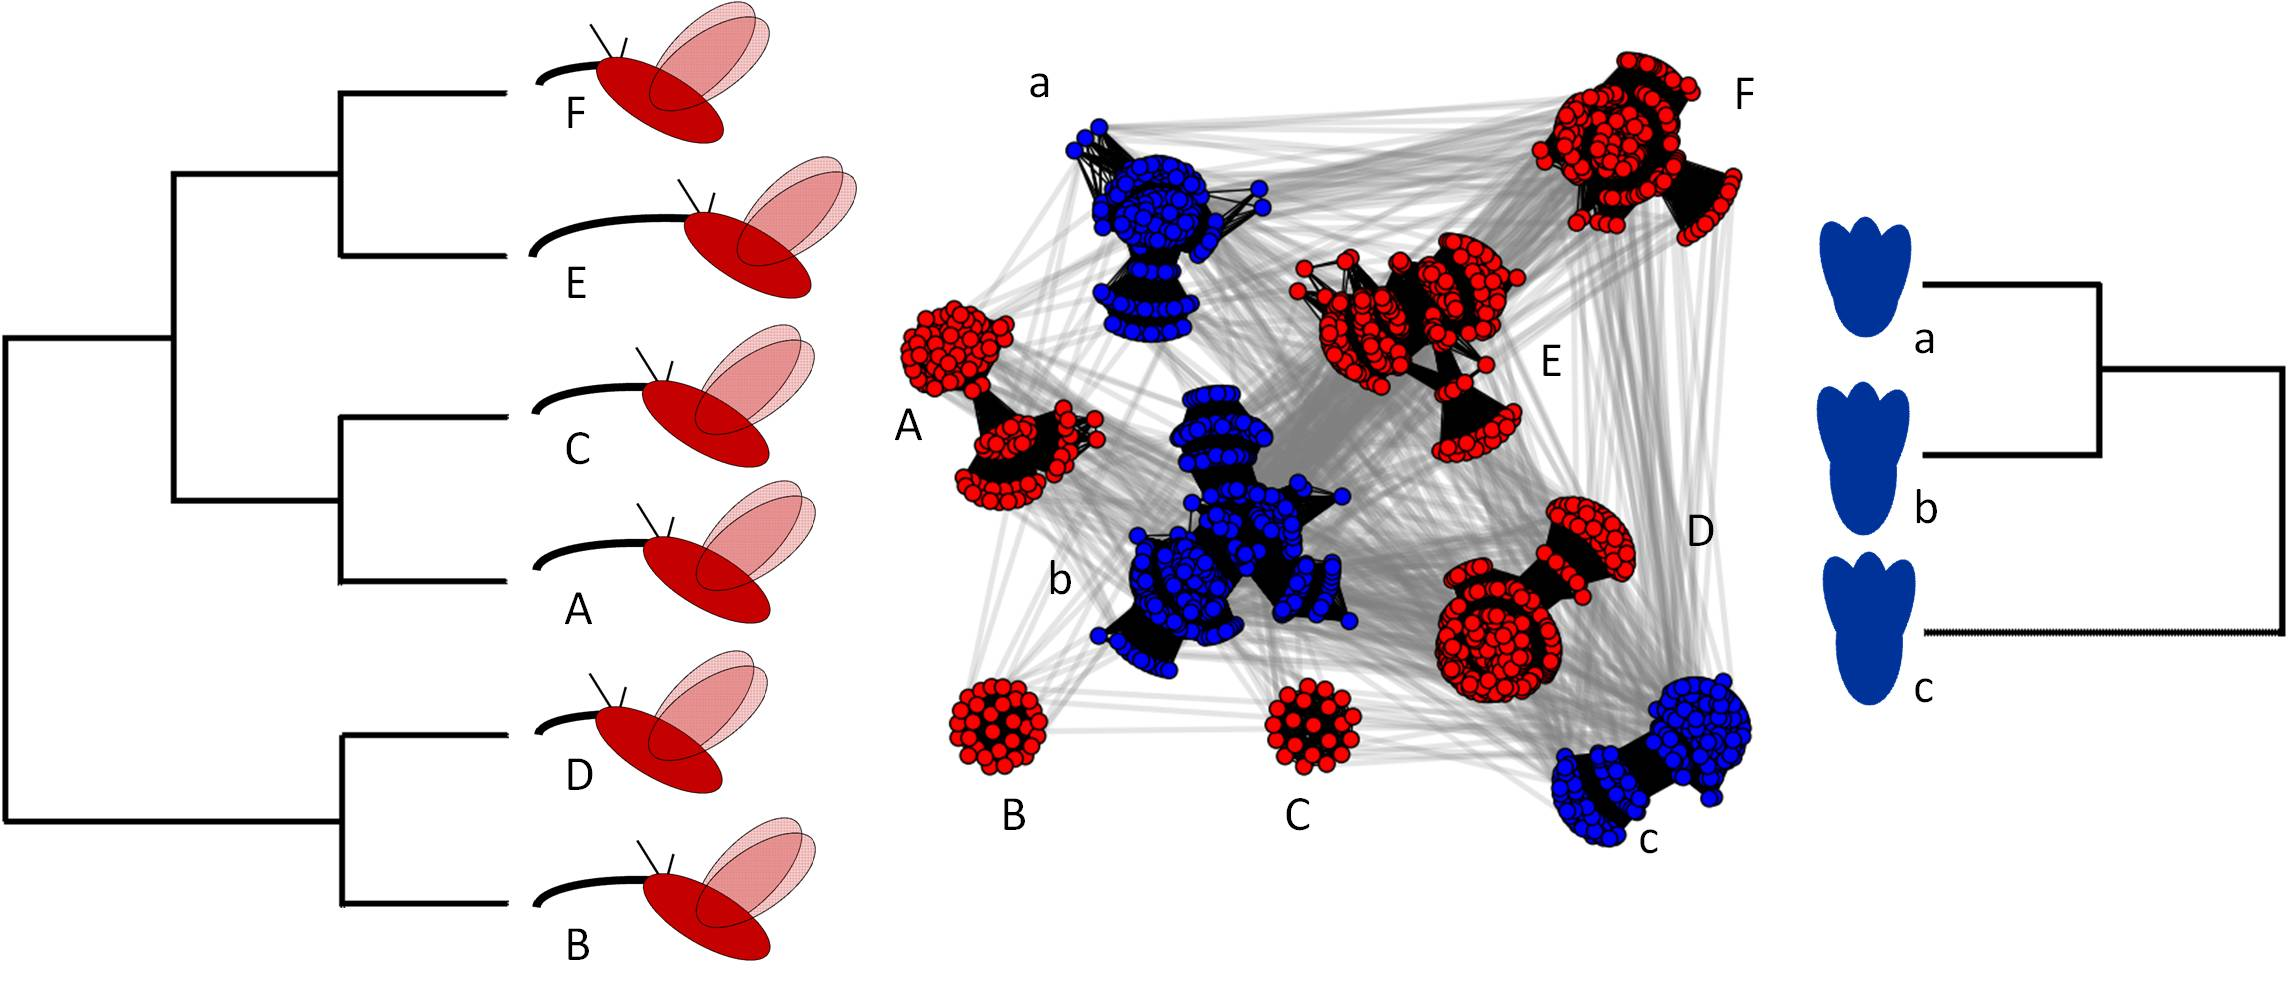
\includegraphics[scale=0.4]{Figures/ConvComp3.eps}
\par\end{centering}

\protect\caption{Evolutionary convergence and complementarity in plant-pollinator networks.
Trees at the left and right side show genetic similarities between
animal (red) and plant (blue) species, respectively. Mean species
trait, proboscis and corolla length, is sketched with cartoons next
to their respective position in the trees. Animals, composed by six
species, have two evolutionary convergence events (A-B and F-D). Plants,
composed by three species, have one convergent event (b-c). The central
part of the figure shows the network of plant-animal interactions,
where each node (colored filled circles) represents an individual.
The network is composed of two types of links: genetic relatedness
links (black solid) forming clusters that represent species and plant-animal
individual-based interaction links (gray). The network shows variability
in terms of genetic relatedness and plant-animal interactions within
a species (i.e. high intraspecific variability). This figure is an
example from one simulation. Parameters used are as in figure 3,\textbf{
$q_{min}=0.97$, $d_{max}=d_{max}^{PA}=0.3$, $\mu=5\times10^{-3}$
and $J^{P}=J^{A}=1,000$.\label{fig:convergence-complementarity}}}


\end{figure}


\begin{figure}
\begin{centering}
\includegraphics[scale=0.6]{Figures/matrixplantperspb0052.eps}
\par\end{centering}
\protect\caption{Plant-animal species interaction network. Plant species are represented
in rows and animal species in columns. The color gradient indicates
the number of mutualistic partners (i.e. individuals interacting)
shared between plant and animal species. This matrix comes from one
replicate with nine plant and thirteen animal species. The network
shows high level of nestedness ($N=0.72$) and intermediate level
of connectance ($C=0.5$). Parameters used are $q_{min}=0.97$, $d_{max}=d_{max}^{PA}=0.3$,
$\mu=5\times10^{-3}$ and $J_{P}=J_{A}=1,000$.\textbf{\label{fig:nestedness}}}


\end{figure}


\begin{figure}
\begin{centering}
\includegraphics[scale=0.7]{Figures/ConvCompFinal.eps}
\par\end{centering}
\vspace{-2.5 in}
\protect\caption{Comparison of model's predictions with estimations of convergence
and complementarity from an empirical data of a plant-pollinator community.
a) The proportion of complementarity events (y-axis) as a function
of the complementarity threshold (x-axis) for the empirical data (dotted
black line) and for the model (continuous and dotted red lines represent
mean, 0.05 and 0.95 CI values, respectively). Predictions are within
the CI for most complementarity threshold values. Empirical data deviates
from model predictions for complementarity threshold values around
0.4 and lower. b) The proportion of convergence events in the plant
community (y-axis, 69 species) as a function of the convergence threshold
(x-axis) for the empirical data (dotted black line) and for the model
(continuous and dotted red lines represent mean, 0.05 and 0.95 CI
values, respectively). Convergence events in the empirical data strongly
deviates from model predictions for convergence threshold values ranging
between 1 and approx. 0.82. In that range, model predicts much higher
proportion of convergence events than the empirical observations.
c) The proportion of convergence events in the animal community (y-axis,
24 species) as a function of the convergence threshold (x-axis) for
the empirical data (dotted black line) and for the model (continuous
and dotted red lines represent mean, 0.05 and 0.95 CI values, respectively).
Convergence events in the empirical data are within the CI of model
predictions for most convergence threshold values. }


\end{figure}


\pagebreak{} 
\end{document}
